%Fiquemos com Deus e Nossa Senhora!
%Sao Jose de Cupertino rogai por nos!!
%Honra teu pai e tua mae!
% ### Uses XeLaTeX ### %
% ### Needs beamer-master ### %
\documentclass[aspectratio=169]{beamer} %. Aspect Ratio 16:9

\usetheme{AI2} % beamerthemeSprace.sty
\usepackage[portuguese]{babel}
\usepackage[utf8]{inputenc}
\usepackage[T1]{fontenc}
\usepackage{ragged2e,bm,oubraces,tikz}
\usepackage{algorithmic}
\usepackage{tikz}

\usetikzlibrary{automata, positioning, arrows}
\DeclareMathOperator*{\argmin}{arg\,min}
\DeclareMathOperator*{\argmax}{arg\,max}

\newcommand*\mycirc[1]{%
  \begin{tikzpicture}
    \node[draw,circle,inner sep=2pt] {#1};
  \end{tikzpicture}}
  
 \newenvironment{algorithm}{\begin{quote} %\vspace{1em}
\begin{algorithmic}\samepage}{\end{algorithmic} %\vspace{1em} 
\end{quote}}

% DATA FOR FOOTER
\date{2025}
\title{- Teoria da Computação e Linguagens Formais}
\author{João Paulo Papa}

\begin{document}
% ####################################
% FIRST SLIDE 						:: \SliTit{This is the Title of the Talk}{A. B. Name}{Sprace}
% SUB-TITLE SLIDE 					:: \SliSubTit{<title>}{<explanation}
% SUB-SUB-TITLE SLIDE				:: \SliSubSubTit{<title>}{<explanation}
% SLIDE WITH TITLE 					:: \SliT{Title}{Content}
% SLIDE NO TITLE 						:: \Sli{Content} 
% SLIDE DOUBLE COLUMN WITH TITLE 	:: \SliDT{Title}{First Column}{Second Column}
% SLIDE DOUBLE COLUMN NO TITLE 		:: \SliD{First Column}{Second Column}
% SLIDE ADVANCED WITH TITLE 			:: \SliAdvT{Title}{Content}
% SLIDE ADVANCED NO TITLE 			:: \SliAdv{Content}
% SLIDE ADVANCED DOUBLE WITH TITLE 	:: \SliAdvDT{Title}{First Column}{Second Column}
% SLIDE ADVANCED DOUBLE NO TITLE 	:: \SliAdvD{First Column}{Second Column}
% SLIDE BLACK						:: \Black{ <Content> }
% SLIDE WHITE						:: \White{ <Content> }
% ITEMIZATION 						:: \begin{itemize}  \iOn{First} \iTw {Second} \iTh{Third} \end{itemize}
% COMMENT TEXT				 		:: \note{<comment>}
% SECTION 							:: \secx{Section} | \secxx{Sub-Section}
% BOLD SPRACE COLOR				:: \bfs{<text>}
% TABLE OF CONTENT					:: \tocitem{<title>}{<content>}
% LEFT ALIGN EQUATION				:: \begin{flalign*}  & <equation> &   \end{flalign*}
% CENTER ALIGN EQUATION	S			:: \begin{gather*} <equations>  \end{gather*}
% SLASH								:: \slashed{<>}
% BAR								:: \barr{<letter>} instead of \bar{<letter>}
% THEREFORE						:: use \portanto (larger and bold}
% 2 or 3 MATH SYMBOLS				:: \overset{<up>}{<down>} &  \underset{<below>}{\overset{<above>}{<middle>}}  
% INSERT TEXT IN FORMULA			:: \ins{<text>}
% EXERCISE							:: \exe{<exercise #>}{<exercise text>}
% SUGGESTED READING BOX			:: \sug{<references>}
% CITATION							:: \cittex{<citation>}
% CITATION DOUBLE COLUMN 			:: \cittexD{<citation>}
% TEXT POSITION						:: \texpos{<Xcm>}{<Ycm>}{<text>} origin = center of slide : x right | y down
% REFERENCE AT BOTTOM  S/D SLIDE		:: \refbotS{<reference>} \refbotD{<reference>}
% HIDDEN SLIDE						:: \hid
% COLOR BOX 						:: \blu{blue} + \red{rec} + \yel{yellow} + \gre{green} + \bege{beige}
% FRAME 							:: \fra{sprace} \frab{blue} \frar{red} + \fray{yellow} + \frag{green}		
% FIGURE 							:: \img{X}{Y}{<scale>}{Figure.png} 
% FIGURE							:: \includegraphics[scale=<scale>]{Figures/.png}
% FIGURE DOUBLE SLIDE NO TITLE		::  \img{-4}{0.5}{<scale>}{Figure.png} % Image 1st half
%									::  \img{4}{0.5}{<scale>}{Figure.png} % Image 2nd half
% FIGURE DOUBLE SLIDE WITH TITLE		::  \img{-4}{0}{<scale>}{Figure.png} % Image 1st half
%									::  \img{4}{0}{<scale>}{Figure.png} % Image 2nd half
% INCLUDING SWF (Flash)				:: \usepackage{media9} and \includemedia >> USE ACROBAT <<
%%%%%%%%%%%%%%%%%%%%%%%%%%%%%%%%%%%%%%%%%%%%%%%%%%
% ###############################################################################
% FIRST SLIDE
\SliTit{Aula 2 - Linguagens Regulares}{Teoria da Computação e Linguagens Formais}{}{João Paulo Papa (UNESP/Bauru)}
%%%%%%%%%%%%%%%%%%%%%%%%%%%%%%%%%%%%%%%%%%%%%%%%%%
% ###############################################################################
% SLIDE SUB-TITLE
%\SliSubTit{Sub-Title}{Description}{}
%%%%%%%%%%%%%%%%%%%%%%%%%%%%%%%%%%%%%%%%%%%%%%%%%%
% ###############################################################################
%\SliSubSubTit{Sub-Sub-Title}{Description}
 %%%%%%%%%%%%%%%%%%%%%%%%%%%%%%%%%%%%%%%%%%%%%%%%%%



\SliT{Agenda}{
\justifying Nesta aula iremos abordar os seguintes assuntos:

\begin{itemize}
	\item Hierarquia de Chomsky.
	\item Linguagens Regulares.
	\item Sistemas de Estados Finitos.
	\item Autômatos Finitos.
\end{itemize}
}

\Sli{
\justifying Noam Chomsky é um cientista norte-americano que classificou as gramáticas em quatro tipos.

\begin{center}
	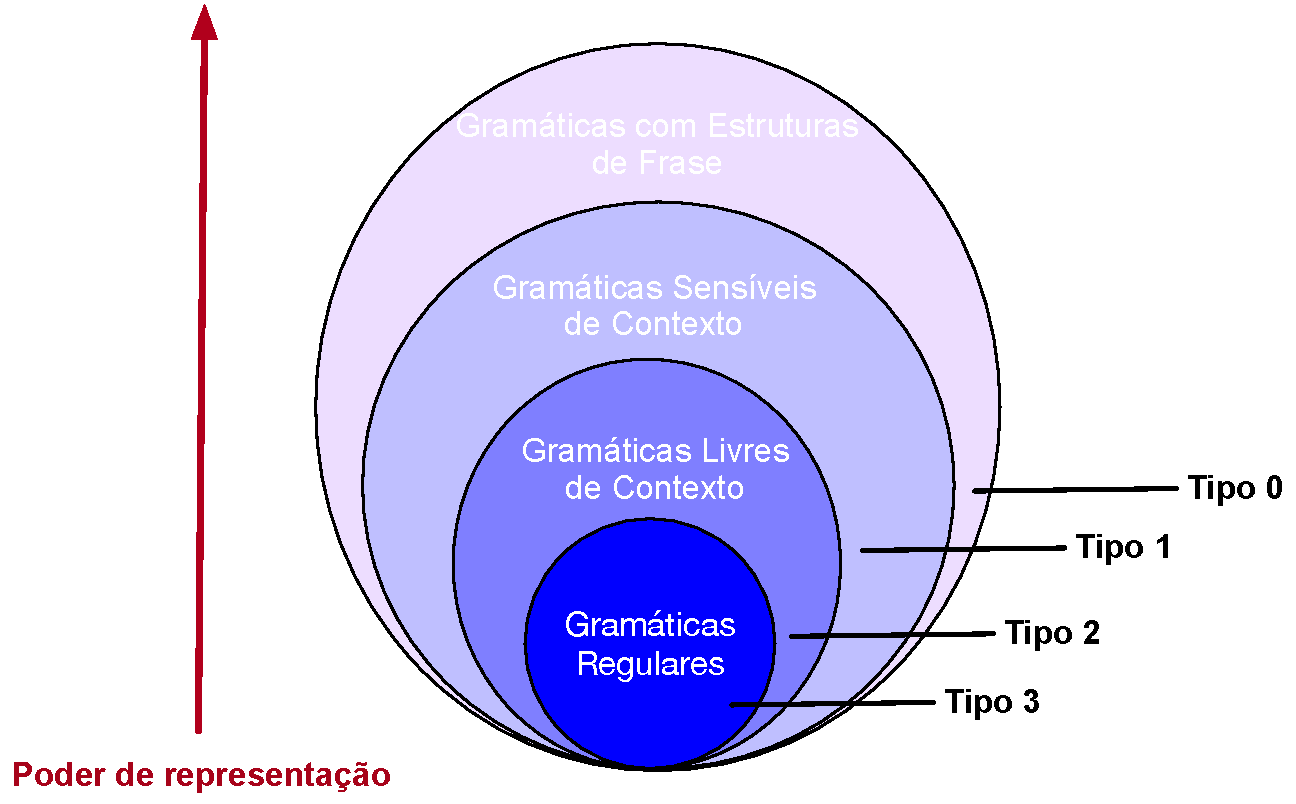
\includegraphics[scale=0.43]{figs/hierarquia_chomsky.pdf}
\end{center}

}

\Sli{
\justifying Cada gramática possui sua \textbf{abstração computacional} para representá-la. Vamos começar pelo tipo 3, ou seja, pelas \textbf{Gramáticas Regulares} (GR), que são as mais simples.\newline

\justifying Uma gramática $G=(V,T,P,S)$ é dita ser regular quando ela obedece às seguintes regras:

\begin{itemize}
	\item Ela é uma \textbf{Gramática Linear à Direita} (GLD) \underline{ou} uma \textbf{Gramática Linear à Esquerda} (GLE).
	\item Uma gramática é GLD quando suas regras de produção $P$ obedecem às seguintes propriedades:\[A\rightarrow aB|a\text{\ \ ou\ \ }A\rightarrow a,\]
	em que $A,B\in V$ e $a\in T$.
	\item Uma gramática é GLE quando suas regras de produção $P$ obedecem às seguintes propriedades:\[A\rightarrow Ba|a\text{\ \ ou\ \ }A\rightarrow a,\]
	em que $A,B\in V$ e $a\in T$.

\end{itemize}
}

\SliT{Linguagens Regulares}{
\justifying Uma linguagem $L$ é regular (LR), ou seja, do tipo 3, se existe, pelo menos, um \textbf{autômato finito determinístico} que a reconhece.\newline

\justifying Estudaremos três tipos de formalismos com relação às Linguagens Regulares:

\begin{itemize}
	\item Autômato Finito.
	\item Expressão Regular.
	\item Gramática Regular.
\end{itemize}
}

\Sli{
\justifying \textbf{Autômato Finito:} é um formalismo \textbf{operacional} ou reconhecedor. Na prática, caracteriza-se como um sistema de estados finitos (similar à um grafo).\newline

\justifying \textbf{Expressão Regular:} é um formalismo \textbf{denotacional} ou gerador.\newline

\justifying \textbf{Gramática Regular:} é um formalismo \textbf{axiomático} ou gerador. Possui, também, restrições na forma de regras de produção.
}

\Sli{
\justifying Algumas características das Linguagens Regulares:

\begin{itemize}
	\item Classe de linguagens mais simples (hierarquia de Chomsky).
	\item Utilizada, principalmente, na análise \textbf{léxica}.
	\item Seu formalismo de reconhecimento (autômato) é, geralmente, fácil de implementar e possui pouca complexidade.
	\item Qualquer autômato finito é igualmente \textbf{eficiente} e \textbf{ótimo} (caso não possua estados \textbf{redundantes}).
\end{itemize}
}

\SliT{Sistema de Estados Finitos}{
\justifying Um Sistema de Estados Finitos possui as seguintes características:

\begin{itemize}
	\item Modelo matemático de sistema com \textbf{entradas} e \textbf{saídas} discretas.
	\item Composto por \textbf{entrada} e \textbf{estados}.
	\item \textbf{Não} tem memória.
	\item Número \textbf{finito} de estados.
	\item A máquina só pode estar em um \textbf{único} estado de cada vez.
\end{itemize}
}

\SliT{Autômato Finito}{
\justifying Um Autômato Finito (AF) é um sistema de estados finitos e podem ser divididos, de maneira geral, em três tipos:

\begin{itemize}
	\item \textbf{Autômato Finito Determinístico (AFD):} a partir de um determinado estado e de um símbolo lido, pode assumir um \textbf{único} estado.
	\item \textbf{Autômato Finito Não Determinístico (AFN):} a partir de um determinado estado e de um símbolo lido, pode assumir um \textbf{conjunto} de estados.
	\item \textbf{Autômato Finito Não Determinístico com Movimentos Vazios (AFN$_\epsilon$):} a partir de um determinado estado e \textbf{sem ler} um símbolo, pode assumir um \textbf{conjunto} de estados.
\end{itemize}
}

\Sli{
\justifying Um Autômato Finito é composto pelos seguintes itens:

\begin{minipage}{0.617\textwidth}
\begin{itemize}
	\item Fita:
	\begin{itemize}
	\item É o dispositivo de entrada.
	\item Possui (armazena) a informação a ser processada.
	\item Não é possível gravar dados.
	\end{itemize}	
	\item Unidade de controle:
	\begin{itemize}
	\item Reflete o estado corrente da máquina.
	\item Possui uma unidade de leitura (cabeça da fita).
	\item Acessa uma célula da fita de cada vez.
	\item Movimenta-se exclusivamente para a direita.
	\end{itemize}
	\item Função programa ou transicão:
	\begin{itemize}
	\item Comanda as leituras.
	\item Define o estado da máquina.
	\end{itemize}
\end{itemize}
\end{minipage}%%% to prevent a space
\begin{minipage}{0.37\textwidth}
\begin{center}
	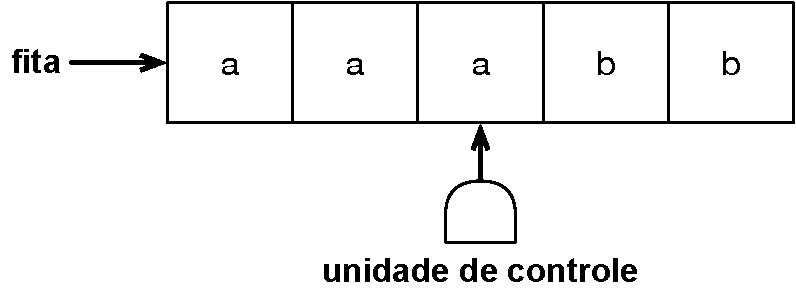
\includegraphics[scale=0.43]{figs/fita.pdf}
\end{center}
\null
\par\xdef\tpd{\the\prevdepth}
\end{minipage}
}

\Sli{
\justifying Como funcionam as funções de transição?\newline 

\begin{minipage}{0.537\textwidth}
\vspace{-1.7cm}
\justifying Suponha a seguinte função: $\delta(p,a)=\{q\}$. \newline Ela nos diz que, se estivermos no estado $p$\\e lermos (consumirmos) o caractere $a$, então\\vamos para o estado $q$.
\end{minipage}%%% to prevent a space
\begin{minipage}{0.37\textwidth}
\begin{center}
	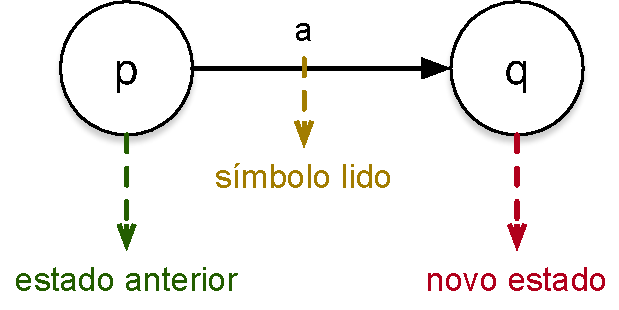
\includegraphics[scale=0.57]{figs/automato_simples.pdf}
\end{center}
\null
\par\xdef\tpd{\the\prevdepth}
\end{minipage}
}

\Sli{
\justifying Formalmente, um AFD é definido pela 5-upla ordenada abaixo:

\begin{equation*}
	M=(\Sigma,Q,\delta,q_0,F),
\end{equation*}
em que:\newline\newline
$\Sigma$: alfabeto de entrada\newline
$Q$: conjunto de estados\newline
$\delta$: função de transição da forma $\delta: Q\times \Sigma\rightarrow Q$\newline
$q_0$: estado inicial tal que $q_o\in Q$\newline
$F$: estado final tal que $F\subseteq Q$
}

\Sli{
\justifying \underline{Exemplo:} construa um AFD $M$ que reconheça a seguinte linguagem $L=\{aa\}$.

\justifying Seja $M=(\Sigma,Q,\delta,q_0,F)$ um AFD que reconhece $L$. Temos que $M$ pode ser definido da seguinte maneira:\newline\newline
$\Sigma = \{a\}$\ \ \ \ $Q=\{q_0,q_1,q_2\}$\newline
$q_0=\{q_0\}$\ \ \ \ $F=\{q_2\}$\newline

\begin{minipage}{0.337\textwidth}
\begin{table}
\begin{tabular}{c|c|}
& $a$ \\\hline
$q_0$ & $q_1$\\
$q_1$ & $q_2$\\
\end{tabular}		
\end{table}

\end{minipage}%%% to prevent a space
\begin{minipage}{0.57\textwidth}
\begin{center}
\begin{tikzpicture}
\node[state, initial, initial text=] (q_0) {$q_0$};
\node[state, right = of q_0] (q_1) {$q_1$};
\node[state, accepting, right = of q_1] (q_2) {$q_2$};

\path[-stealth, thick]
	(q_0) edge[above] node {a} (q_1)
	(q_1) edge[above] node {a} (q_2);

\end{tikzpicture}
\end{center}

\null
\par\xdef\tpd{\the\prevdepth}
\end{minipage}
}

\Sli{
\justifying \underline{Exemplo:} construa um AFD $M$ que reconheça uma linguagem $L$ que contenha $aa$ como subpalavra.

\justifying Seja $M=(\Sigma,Q,\delta,q_0,F)$ um AFD que reconhece $L$. Temos que $M$ pode ser definido da seguinte maneira:\newline\newline
\vspace{-1cm}
\begin{minipage}{0.377\textwidth}
$\Sigma = \{a,b\}$\ \ \ \ $Q=\{q_0,q_1,q_2\}$\newline
$q_0=\{q_0\}$\ \ \ \ $F=\{q_2\}$\newline

\begin{table}
\scalebox{0.7}{
\begin{tabular}{c|c|c|}
& $a$ & $b$\\\hline
$q_0$ & $q_1$ & $q_1$\\
$q_1$ & $q_2$ & $q_0$\\
$q_2$ & $q_2$ & $q_2$\\
\end{tabular}}		
\end{table}

\end{minipage}%%% to prevent a space
\begin{minipage}{0.57\textwidth}
\begin{center}
\begin{tikzpicture}
\node[state, initial, initial text=] (q_0) {$q_0$};
\node[state, right = of q_0] (q_1) {$q_1$};
\node[state, accepting, right = of q_1] (q_2) {$q_2$};

\path[-stealth, thick]
	(q_0) edge[loop above] node {b} (q_0)
	(q_0) edge[bend left, above] node {a} (q_1)
	(q_1) edge[bend left, below] node {b} (q_0)
	(q_1) edge[above] node {a} (q_2)
	(q_2) edge[loop above] node {a,b} (q_2);
	
\end{tikzpicture}
\end{center}\null
\par\xdef\tpd{\the\prevdepth}
\end{minipage}
}

\Sli{
\justifying Não existem regras para a construção de autômatos. Devemos usar nossa experiência e também com base na ``tentativa e erro".\newline\newline

\justifying Um autômato $M$ aceita uma linguagem $L$ quando, dada uma palavra $w\in L$, $M$ pára em um \textbf{estado final} e lê a \textbf{sequência toda}.
}
\end{document}